% General review of all topics
% Emphasis on: Branching, Loops, Functions, Mutability & Python Memory Model
% Brief review of lists, strings, tuples, sets, dictionaries
% Emphasis on: File I/O, Error handling, Classes & Inheritance

% created by Uwe Schadewald
% modified by Mathias Kuntze and Ahmet Uysal
% Add, handout to documentclass arguments for condensed pdf
\documentclass[presentation, 8pt, mathserif, t]{beamer} % , aspectratio=169
\usepackage[english]{babel}
\usepackage{pgf,graphicx}
\usepackage{amsmath, amssymb}
\usepackage[utf8]{inputenc}
\usepackage{lmodern}
\usepackage{palatino}
\usepackage{multimedia}
\usepackage{pgfpages} 
\usepackage{tikz}
\usepackage{datetime}
\pdfoptionpdfminorversion=5

\usepackage{caption}
\usepackage{subcaption}
% if else
\usepackage{ifthen}
% extend table options
\usepackage{tabularx} 
\usepackage{booktabs}
\usepackage{multicol}
\usepackage{multirow}
\usepackage{eso-pic}  % package to set background image
\usepackage[calc]{picture}

% Packages and stuff for ToDo list like itempoints
\usepackage{pifont}
\newcommand{\cmark}{\ding{51}}%
\newcommand{\xmark}{\ding{55}}%
\newcommand{\open}{$\square$}
\newcommand{\done}{\rlap{$\square$}{\raisebox{1pt}{\large\hspace{1.5pt}\cmark}}\hspace{-2.5pt}}
\newcommand{\wontfix}{\rlap{$\square$}{\raisebox{1pt}{\large\hspace{1.5pt}\xmark}}}
\newcommand{\notsure}{\rlap{$\square$}{\raisebox{0.8pt}{\large\hspace{1.5pt}\textbf{?}}}}



% side bar and footer
\setbeamertemplate{headline}{	
	\leavevmode
	\vspace{-4em}	
	\hbox{		
		\begin{beamercolorbox}[wd=0.85\paperwidth,ht=10ex,dp=8ex,center]{}%			
			% navigation with subsections as dots
			\hspace{3.5em}\insertnavigation{0.7\paperwidth}{\hskip0pt plus1fill} % add navigation in footer						
			% navigation with sections, no subsections
			% \insertsectionnavigationhorizontal{0.6\paperwidth}{\hskip0pt plus1fill}{} \\ % add navigation in footer}
			
		\end{beamercolorbox} 				
	}
	\vskip0pt
}


\setbeamertemplate{footline}{	
	\leavevmode
	\vspace{-3em}
	\hbox{
		\begin{beamercolorbox}[wd=.33\paperwidth,ht=2.25ex,dp=1ex,left]{author in head/foot}%
			\hspace{5em}
			\insertshortauthor
		\end{beamercolorbox}
		\begin{beamercolorbox}[wd=.33\paperwidth,ht=2.25ex,dp=1ex,center]{title in head/foot}%
			\insertshorttitle \ - \insertshortsubtitle
		\end{beamercolorbox}	
		\begin{beamercolorbox}[wd=0.30\paperwidth,ht=10ex,dp=8ex,right]{pagenumber in head/foot}			 	
			\insertframenumber % add page numbers
		\end{beamercolorbox}
	}			
	\vskip0pt
}



\setbeamertemplate{frametitle}{
	\ifthenelse{\equal{\insertframesubtitle}{}}{
		\vspace{0.6cm}
		\huge{\insertframetitle}
	}{
		\vspace{0.6cm}
		\small{\insertframetitle}\\
		\vspace{0.3cm}
		\huge{\insertframesubtitle}
    }		
}

	
% enumerate sections
\setbeamertemplate{section in head/foot}{\hfill\insertsectionheadnumber.~\insertsectionhead}
%\setbeamertemplate{section in head/foot shaded}{\color{structure!50}\hfill\insertsectionheadnumber.~\insertsectionhead}
\setbeamertemplate{section in toc}{\inserttocsectionnumber.~\inserttocsection}

%enumerate subsections
\setbeamertemplate{subsection in head/foot}{\hfill\insertsubsectionheadnumber.~\insertsubsectionhead}
\setbeamertemplate{subsection in head/foot shaded}{\color{structure!50}\hfill\insertsubsectionheadnumber.~\insertsubsectionhead}
%\setbeamertemplate{subsection in toc}[subsections numbered]
\setbeamertemplate{subsection in toc}{\vskip0.5em\leftskip=2em\inserttocsubsection\par}

%--------------------------Common------------------------------------------------------
\setbeamercovered{transparent} % make the beamer theme invisible
\usefonttheme{structurebold}
\beamertemplatenavigationsymbolsempty % set navigations helper function to off
\setbeamertemplate{bibliography item}[text]
\setbeamertemplate{note page}[plain]

%\setlist[itemize,1]{label={$\bullet$}} % \item are using bullets
\setbeamertemplate{itemize items}[circle]
	
	

	
% create a new command to show it on two screens
% I'm using dspdfviewer.
\newcommand{\setDualView} {
	\setbeameroption{show notes on second screen=right}
}

%\AtBeginSection[]{\subsection{}}
\newcommand{\addcite}[1]{%
	\AddToShipoutPictureFG*{%
		\AtPageLowerLeft{%
			\put(0.90\paperwidth,5em){											
				\tiny{
					\cite{#1} 
				}			
			}
		}
	}	
}

% insert a frame with references -> use bibtex
\newcommand{\insertReferenceFrame}[3]{%
	\section{#1}
	\begin{frame}[allowframebreaks]
		\frametitle{#1}
		\bibliographystyle{#2}
		\bibliography{#3}
	\end{frame}	
}

\AtBeginSection[]{\subsection{}}
	





\usepackage{../KU-Beamer-Template/style/koc} 
\usepackage{minted}
\usepackage{upquote}
\usepackage{graphicx}

\title{KOLT Python}
\subtitle{Third-Party Packages} 
\newdate{date}{22}{04}{2019}
\date{\displaydate{date}}
\author{Ahmet Uysal}

\titlegraphic{
\includegraphics[scale=0.2]{../KU-Beamer-Template/style/images/logo_kolt.eps}}

\setbeamercovered{invisible} % transparent

\begin{document}
    \maketitle

    \frame{\frametitle{Agenda}\tableofcontents}

    \section{Package Management}

    \begin{frame}
        \frametitle{Python Package Index (PyPI)}
        \pause
        \huge
        Repository of software for the Python programming language.
        \pause
        \begin{itemize}
            \item 23,000+ Python3 packages.
            \pause
            \item If you want a package, PyPI probably has it. 
        \end{itemize}
    
    \end{frame}

    \begin{frame}
        \frametitle{pip}
        \LARGE
        \pause
        \begin{itemize}
        \item Recommended tool for installing Python packages.
        \pause
        \item \textbf{\texttt{pip}} is already installed with modern Python distributions.
        \pause
        \item Try \texttt{pip -V} on your command line/terminal(\texttt{pip3 -V} for Macs). 
        \end{itemize}
        \pause
        \texttt{\$ pip -V}\\
        \texttt{pip 19.0.3 from --PATH\_TO\_PIP-- (python 3.7)}\\
        \pause
        \begin{center}
            \huge
            \textbf{Any problems?}            
        \end{center}
        
    \end{frame}

    \begin{frame}
        \frametitle{Common pip commands}
        \LARGE
        \pause
        \textbf{Install a package:}\\
        \pause
        \texttt{\$ pip \textbf{install} package\_name}  \# latest version \\
        \pause
        \texttt{\$ pip \textbf{install} package\_name==1.0.1}  \# specific version \\
        \pause
        \texttt{\$ pip \textbf{install} package\_name>=1.0.1}  \# minimum version \\
        \pause        
        \textbf{Uninstall a package:}\\
        \pause        
        \texttt{\$ pip \textbf{uninstall} package\_name}\\
        \pause
        \textbf{Update a package:}\\
        \pause
        \texttt{\$ pip \textbf{install --upgrade} package\_name}\\
        \pause
        \textbf{Search PyPI for matches:}\\
        \pause
        \texttt{\$ pip \textbf{search} query}
    \end{frame}

    \section{Solving a Real Life Problem}

    \begin{frame}
        \frametitle{Solving a Real Life Problem}
        \pause
        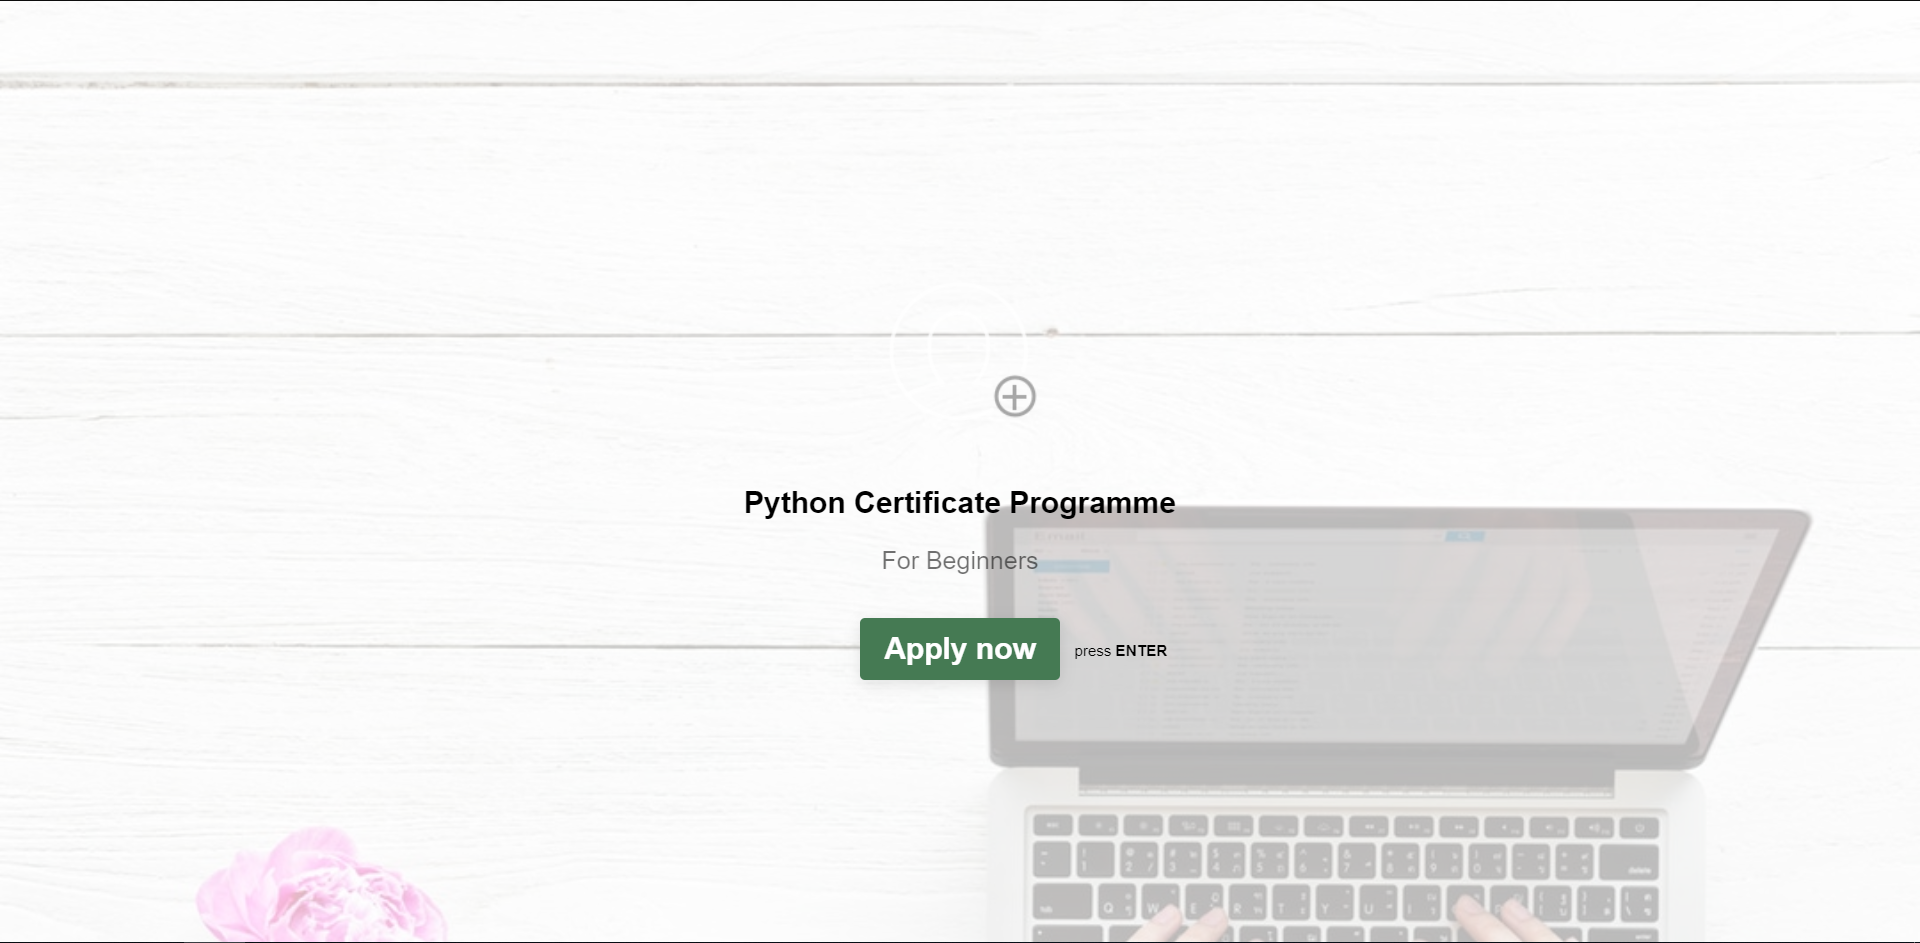
\includegraphics[height=0.7\textheight]{images/typeform.PNG}
    \end{frame}

    \begin{frame}
        \frametitle{Problems}
        \LARGE
        \pause
        \begin{itemize}
            \item No option for Masters/PhD levels
            \pause
            \item No standard for study areas(majors)
            \pause
            \item \textbf{What do you study in Koç?}
            \pause
            \begin{itemize}
                \large
                \item Business Administration
                \pause
                \item Bussines Administratiom
                \pause
                \item Business
                \pause
                \item BA
                \pause
                \item \dots
            \end{itemize}
        \end{itemize}
        \pause
        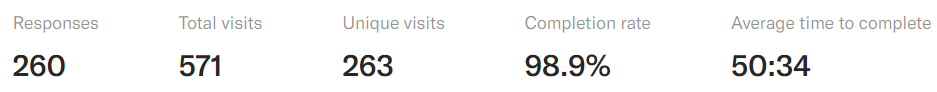
\includegraphics[width=0.7\textwidth]{images/stats.PNG}
    \end{frame}

    \begin{frame}
        \frametitle{How to Categorize Students?}
        \LARGE
        We need academic level and major statistics of applicants.\\
        \pause 
        What can we use?
        \begin{itemize}
            \pause
            \item Jokes?
            \pause
            \item Student mails?
            \pause
            \item KU usernames?
        \end{itemize}
        \pause
        \texttt{ldap.ku.edu.tr}
    \end{frame}

    \begin{frame}
        \frametitle{How to Categorize Students?}
        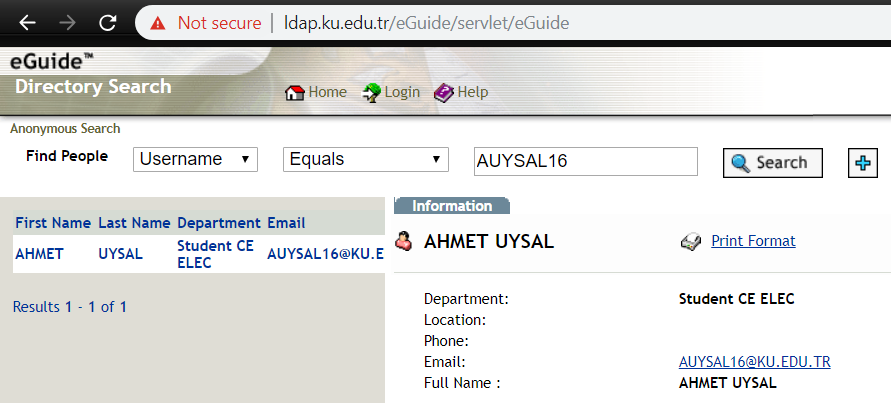
\includegraphics[width=0.7\textwidth]{images/ldap_auysal16.PNG}
    \end{frame}

    \begin{frame}
        \frametitle{Where did this information come?}
        \LARGE
        \begin{itemize}
            \pause
            \item Open the \textbf{developer console} on your browser.
            \pause
            \item Windows: \texttt{Ctrl+Shift+I}, Mac: \texttt{Option+Command+I}
            \pause
            \item Go to \textbf{network} tab.
            \pause
            \item Search for a person.
        \end{itemize}
        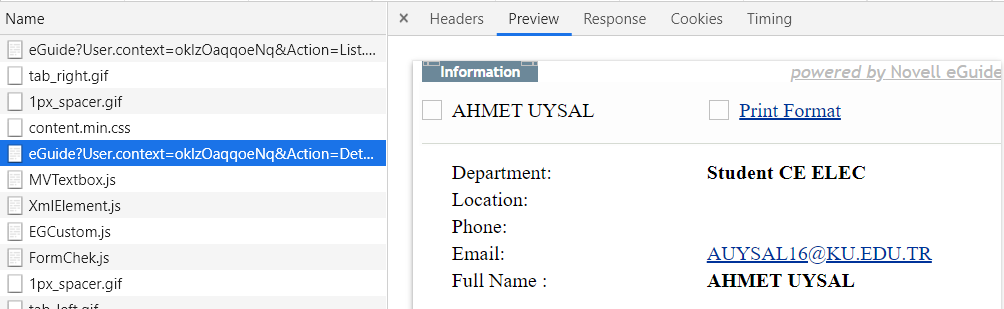
\includegraphics[width=0.7\textwidth]{images/ldap_network.PNG}

    \end{frame}

    \begin{frame}
        \frametitle{HTTP Requests}
        \LARGE
        \pause
        Your browser sent a HTTP \textbf{GET} request to \texttt{http://ldap.ku.edu.tr/eGuide/servlet/eGuide} to get the data.\\
        \pause
        Examine the request using a tool like Postman.\\
        \pause
        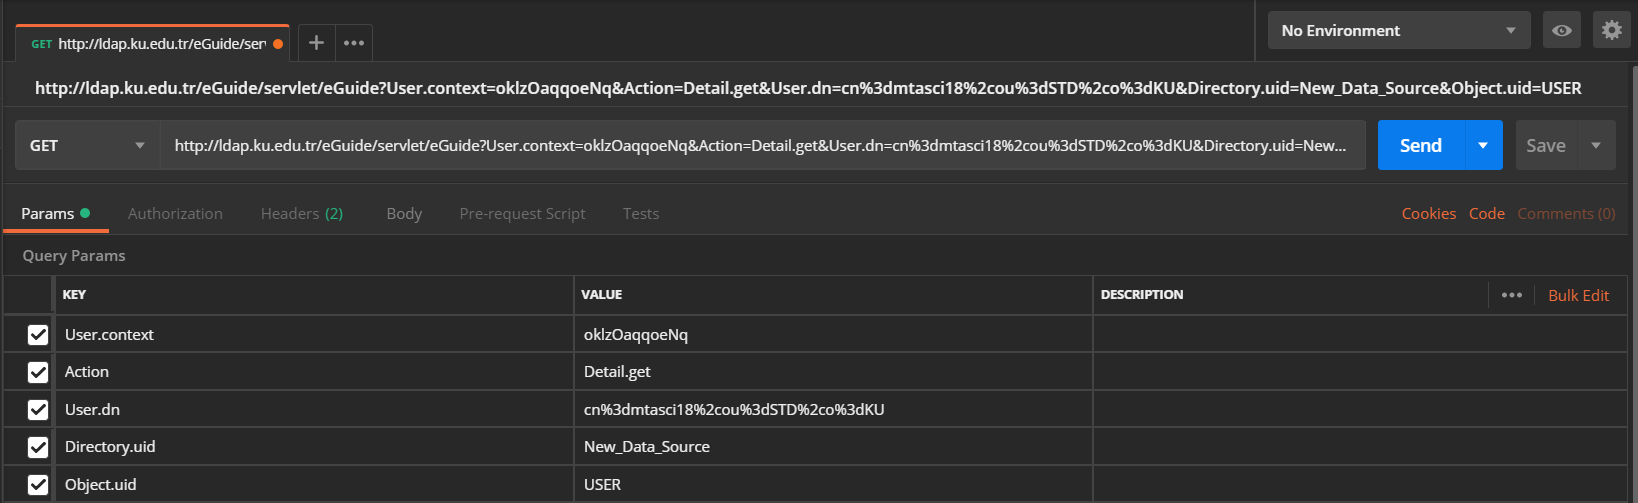
\includegraphics[width=0.55\textwidth]{images/postman.PNG}
        \pause
        \\Can we send this request programmatically?
    \end{frame}

    \begin{frame}
        \frametitle{requests package}
        \LARGE
        \texttt{\textbf{requests}}: HTTP for Humans\\
        \pause
        install using \texttt{\textbf{pip}}: \texttt{\$ pip install requests}\\
        \pause
        \href{https://2.python-requests.org/en/master/user/quickstart/}{\underline{\textit{requests Quickstart}}}
        \pause
        \inputminted[frame=single,framesep=2pt]{python3}{code-examples/req.py}
    \end{frame}

    \begin{frame}
        \frametitle{import Statements}
        \Large
        \inputminted[frame=single,framesep=2pt]{python3}{code-examples/import_statements.py}

    \end{frame}

    \begin{frame}
        \frametitle{Problem Solution}
        \huge
        You can get the source code \href{https://github.com/koltpython/python-slides/tree/master/Lecture8/code-examples/}{\underline{\textit{here}}}.\\
        \pause
        Solution will be discussed during class time, you can ask your questions with email if you missed the class.
    \end{frame}

    \section{Final Project}
    \begin{frame}
        \frametitle{Final Project}
        \LARGE
        \pause
        Final project is on!
        \pause
        \begin{itemize}
            \item You will work as teams of 2 or 3.
            \pause
            \item You can choose any topic, might be related to your research/other courses
            \pause
            \item Choose something you will enjoy working on
            \pause
            \item We will spend most of our remaining class time working on your projects
            \pause
            \item Proposals due next Monday!
        \end{itemize}
    
    \end{frame}

\end{document}